
\section{Model}
	
	- Network layout 
	
\begin{figure}[H]\centering
	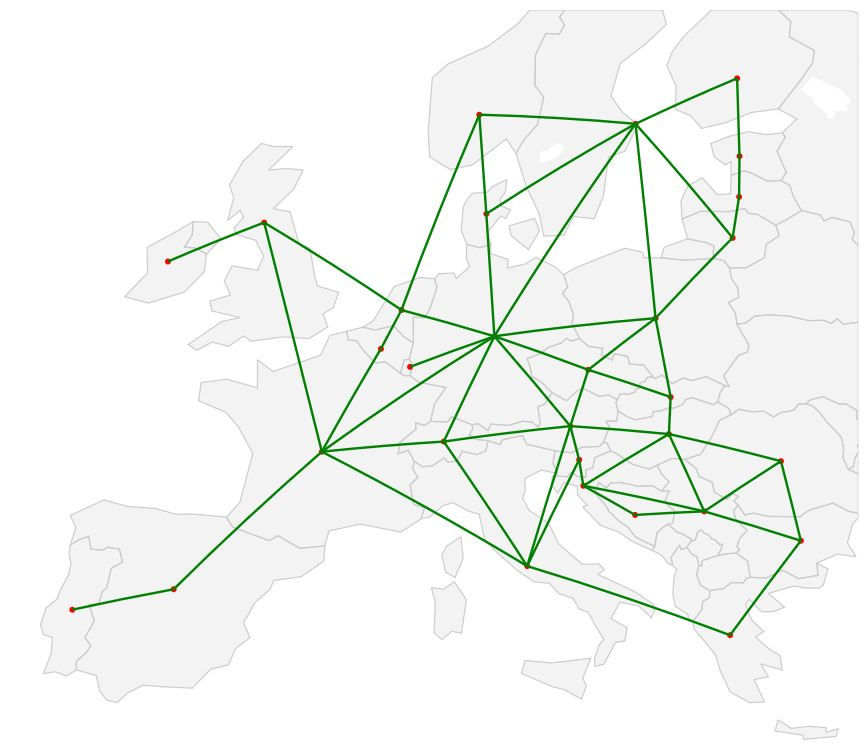
\includegraphics[width=0.95\textwidth]{./Images/network_layout}
	\caption{Network layout}
	\label{fig:network_lay}
\end{figure}
	
\section{The optimization problem}\label{sec:OptimizationProblem}


The optimization problem at hand is a simplified energy economic model of Europe, build with focus on exploring the composition of VRES (variable renewable energy sources) on a global and national scale. In the model each country is represented as a note connected to the surrounding countries through a link. Each country has three energy producing technologies available, gas, wind and solar power. A data resolution of 1 hour is used, and simulations run over an entire year. 

Following the naming convention from \cite{PyPSA_euro_30_model}, indexing the notes in the network with the variable $n$, the power generating technologies by $s$, the hours in the year by $t$ and the possible connecting power lines by $l$, the contributing variables to the objective function describing the total annualized system cost is the following: 

\begin{itemize}
	\item Hourly dispatch of energy from the given plants in the given countries $g_{n,s,t}$ with the marginal cost $o_{n,s}$.
	\item Total installed capacity of the given technologies in the given countries $G_{n,s}$ with the capital cost $c_{n,s}$.
	\item Total installed transmission capacity for all lines $F_{l}$ with the fixed annualized cost $c_{l}$.
	
\end{itemize}

The objective function for the optimization problem then becomes: 

\begin{equation}
min \left( \sum_{n,s} c_{n,s} G_{n,s} + \sum_l c_l F_l + \sum_{n,s,t} o_{n,s} g_{n,s,t} \right)
\end{equation}{}

This objective function is subject to a range of constraints ensuring realistic behavior of the system. As described in \cite{PyPSA_euro_30_model} a power balance constraint is issued to ensure stable operation of the network. These constraints force the sum of energy produced and consumed in every hour to equal zero. The hourly electricity demand at each node is described by $d_{n,t}$, the incidence matrix describing the line connections is given by $K_{n,l}$ and the hourly transmission in each line is described as $f_{l,t}$. Then the power balance constraint becomes:

\begin{equation}
\sum_s g_{n,s,t} - d_{n,t} = \sum_l K_{n,l} f_{l,t} \; \forall n,t
\end{equation}

For all conventional generators the maximum hourly dispatch of energy is limited by the installed capacity. It is important to node that for all simulations performed in this project the installed capacity is a variable. 

\begin{equation}
0\leq g_{n,s,t} \leq G_{n,s} \; \forall n,s,t
\end{equation}

The dispatch of variable renewable energy sources (wind and solar) is not only limited by the installed capacity, as availability, hence the name, is variable. Therefore the constraint for dispatch of variable renewable energy sources become:

\begin{equation}
0 \leq g_{n,s,t} \leq \overline{g}_{n,s,t} G_{n,s} \; \forall n,s,t
\end{equation}

Where $\overline{g}_{n,s,t}$ represents the normalized availability per unit capacity. 

The installed capacity is constrained by the geographical potential calculated in \cite{PypsaModel}.

\begin{equation}
0 \leq G_{n,s} \leq G_{n,s}^{max} \; \forall n,s
\end{equation}

All transmission lines in the model modelled with a controllable dispatch constrained by the fact that there must be energy conservation at each node the line is connected to. !! Something here about which lines is included !!!! . Furthermore the transmission in each line is limited by the installed transmission capacity in each line. 

\begin{equation}
|f_{l,t}| \leq F_l \; \forall l,t
\end{equation}

In the model it is possible to activate a CO2 constraint, limiting the allowed CO2 emissions for the entire energy network. As in \cite{PypsaModel} the constraint is implemented using the specific emissions $e_s$ in CO2-tonne-per-MWh of the fuel for each generator type $s$, with the efficiency $\eta_s$ and the CO2 limit $CAP_{CO_2}$. 

\begin{equation}
\sum_{n,s,t} \frac{1}{\eta_s}g_{n,s,t} e_s \leq CAP_{CO_2}
\end{equation}

The model is implemented in the open source software PyPSA \cite{Pypsa}, using much of the software presented in \cite{PypsaModel}. Optimization of the model is performed with the optimization software Gurobi \cite{Gurobi}. 

\section{Properties of the near optimal feasible space}\label{sec:properties_of_hull}

Analyzing the original optimization problem one can deduct that the feasible decision space, must be convex, as all constraints $f_i$ and the objective function $f_0$ satisfy equation \vref{eq:convex_requirement}, and therefore must be convex \cite{ConvexOpimization}. 

\begin{equation}\label{eq:convex_requirement}
f_i(\alpha x + \beta y) \leq \alpha f_i(x) + \beta f_i(y) \; \forall \; x, y \in \mathbb{R}^n and  \; \alpha, \beta \in \mathbb{R}
\end{equation}

Furthermore, when all variables are bounded; hourly production by the power balance constraint and installed capacity by geographical potential, the feasible decision space is not only convex but also closed. If the geographical potential constraint is excluded the feasible decision space becomes an open convex space as illustrated on \vref{fig:sketch_feasable_space}, this does however not have any immediate consequences, as the objective function increases as one moves in the open direction of the space. 

\begin{figure}[ht]
	\centering
	\incfig{Feasible-space}
	\caption{A sketch of a one dimensional feasible space with MGA constraint }
	\label{fig:sketch_feasable_space}
\end{figure}

\begin{equation}
W = \{ \vec{x}\in \mathbb{R}^d | f_i(x) \geq 0 \}
\end{equation}
!!! This is not completly right !!! 


It is important to note that the variables $\vec{x}$ that defines the decision space in the original solutions are, all hourly technology dispatches $g$, all installed capacities $G$ and all installed line capacities $F$. 

\begin{equation}
\vec{x} = \{g_{n,s,t} \wedge G_{n,s} \wedge F_l \; \forall \; n,s,t,l \}
\end{equation}

Therefore, the dimensionality, of the decision space must be given by the number of nodes in network $n$ for every technology $s$ for every hour $t$, plus the number of nodes $n$ times technologies $s$ and finally the number of lines $l$  \vref{eq:dimentionality}.

\begin{equation}\label{eq:dimentionality}
d = n\cdot s \cdot t + n\cdot s + l
\end{equation}


In the case of the reference model used in this project that gives 
$ 30 \cdot 3 \cdot 8765 + 30 \cdot 3 + 90 = 789030$ 
!!! number of lines is a guestimate!!

The true dimensionality might be lower, as some variables do have strong corelations. 

\subsection{Sub space}

As the dimensionality of the decision space is very large, and therefore becomes very unhandy to work with, it makes sense to look at a subspace of lower dimensionality. One could choose to ignore the hourly dispatch of energy from the individual generators, hereby reducing the dimensionaly by a substantial amount. 

\begin{equation}
d^* = n\cdot s + l
\end{equation}

In that case the dimensionality would only be $d^* = 30\cdot 3 + 90 = 180$. 

The subspace would then be given by:

\begin{equation}
W^* = \{\vec{x}^* \in \mathbb{R}^{d^*} |    \}
\end{equation}

The set $W^*$ therefore includes information about installed capacities of all technologies and transmission lines. Since plant operation, is not the focus of this project, but rather distribution of capacities,  the subspace $W^*$ still provides the information of interest, despite its much lower dimensionality. 

\subsubsection{Further reduction}
If desired it is possible to further reduce dimensionality, by sacrificing all spatial information.

\begin{equation}
x^{**} = \{\sum_n G_{n,s} \forall n,s  \}
\end{equation} 

\begin{equation}
d^{**} = s
\end{equation}

\begin{equation}
W^{**} = \{\vec{x}^{**} \in \mathbb{R}^{d^{**}} |    \}
\end{equation}



\section{Modeling to Generate Alternatives (MGA)}\label{sec:MGA}
In this section the basic principles of MGA will be explained together with the benefits and challenges this technique introduces. 

\subsection{Motivation for using MGA}

In the field of mathematical modeling, the scientist aim to produce models representing physical systems as realistically as possible. However, some degree of uncertainty in the models is inevitable as model fidelity is limited by a range of factors including: numeric precision, uncertainty of data, model resolution etc. Modeling of energy systems is a field especially prone to large model uncertainties, deriving not only from lack of fidelity, but from factors such as unmodeled objectives and structural uncertainty \cite{DeCarolis_MGA}. 

The MGA approach was first introduced in 1982 by Brill et al. \cite{Brill_MGA_1982}, in the field of operations research/management science. This is a field where unmodeled objectives and structural uncertainty, are highly influential. 

!! CITATION !!
The basic insight can be
summarized as follows: Because it is not possible to develop a complete
mathematical representation of complex public planning problems,
structural uncertainty in optimization models will always exist. As a
result, the ideal solution is more likely to be located within the model's
inferior region rather than at a single optimal point or along the noninferior frontier (Brill, 1979)

Policy makers often have strong concerns outside the scope of most models
(e.g., political feasibility, permitting and regulation, and timing of
action), which implies that feasible, suboptimal solutions may be
preferable for reasons that are difficult to quantify in energy economy
optimization models.

The purpose of MGA is to efficiently search the feasible
region surrounding the optimal solution to generate alternative
solutions that are maximally different. !!!

\subsection{Technical explanation of MGA HSJ}

The MGA technique was first introduced in 1982 by Brill et. al in the article \cite{Brill_MGA_1982} and later rediscovered by DeCarolis in \cite{DeCarolis_MGA} for use in energy system optimization. The tecnique lets the user search the near optimal feasible decision space for an optimization problem such as the one addressed in this project described in \ref{sec:OptimizationProblem}. 

In section \ref{sec:OptimizationProblem} a series of constraints bounding the network model is listed. Together these constraints form a feasible region that can be described as a convex set in a $d$ dimensional space. Where d is the number of variables in the model. The feasible set is convex as all bounding constraints are linear. The fact that linear constraints form a convex set is shown in \cite{ConvexOpimization}. The MGA technique introduces yet another constraint limiting the size of this convex set even further by limiting the objective function value of all feasible points to be within a certain range of the optimal solution. The goal of the MGA technique is to explore a finite set of alternative solutions located within this convex set. 

In the orginal articel by Brill et. al \cite{Brill_MGA_1982} the HSJ MGA technique is descrbed with the following steps. 

(1) obtain an initial optimal solution for the problem at hand; (2) define a target value for the objective function by adding a user specified amount of slack to the value of the objective function in the initial solution (3) introduce the constraint limiting the objective function to surpass this target value, to the model (4) formulate a new objective function that seeks to minimize the sum of decision variables that had non zero values in the previous solution of the problem (5) iterate the reformulated problem, updating the objective function every time (6) terminate the optimization when the new solution is similar to or close to any previously found solution. Step 3 and 4 was described mathematically in \cite{Brill_MGA_1982} as follows:

\begin{equation}
\begin{split}
Minimize :&  p = \sum_{k \in K} x_k \\
Subject to :&  f_j(\vec{x}) \leq T_j \forall j  \vec{x}\in X
\end{split}
\end{equation}

In this formulation $k$ represents the variable indices for the variables with nonzero values in the previous solution, $j$ is the objective function indices if multiple objective functions exists, $f_j(\vec{x})$ is the evaluation of the $j$'th objective function and $T_j$ is the target value specified for the particular objective function. In the formulation of the constraint $\vec{x}\in X$ specifies that all previously defined constraints still applies as all new solutions $\vec{x}$ must be a part of the set of feasible solution vectors from the original formulation $X$.

How the new objective function precisely is formulated and which variables to include is discussed in \cite{DECAROLIS2016}, where two alternative approaches of defining the new objective function is presented. One approach suggest giving all nonzero variables from the last iteration a weight of 1 in the new objective function. This approach does not consider weight from previous iterations. However, the second approach suggests adding on to the coefficient with a factor of +1 for every time one variable has appeared with nonzero in a row, hereby further increasing the intended to reduce the use of that specific technology. This 



\subsection{Other MGA approaches}

\section{Novel MGA approach}

In this section a novel approach towards MGA optimization of energy networks will be presented. Based on the same concepts as presented in \ref{sec:MGA} this method seeks to explore not only a few alternative solutions from the decision space, but the entire decision space. Hereby an in depth knowledge of the possible solution is obtained providing insight in the distribution of alternative solutions.

An important feature about the method developed is that it can be used for any dimensional decision space. 

The method developed can be divided into two phases. In the first phase, the shape of the feasible near optimal decision space is found, and in the second phase relevant data is extracted from the found space. 

\subsection{Decision space mapping}
As explained in section \vref{sec:properties_of_hull}, the near optimal feasible space will always be convex, and can either be closed or not. However, when the MGA constraint from equation \vref{eq:MGA_constraint} is introduced the space will be closed. 

\begin{equation}\label{eq:MGA_constraint}
f(\vec{x}) \leqslant f(\vec{x}^*) \cdot (1+\epsilon)
\end{equation}

As we now have a closed convex space, it now is possible to explore the shape of this convex set. Assuming that all constraints used including the MGA constraint is linear, the convex set must be a polyhedral and therefore it is possible to define the shape of this set with a finite number of vertexes. !!! This might not be the case for CO2 constraint!!!! \\

However, finding these vertices is no trivial task. In the method developed, all solutions found, that lie within the near optimal feasible space is treated as a point in that space. Furthermore, the possibility of letting the objective function search in a given direction in the decision space is utilized, by replacing the original objective function to an objective function on the from presented in \vref{eq:objective_func_face_normal}.

\begin{equation}\label{eq:objective_func_face_normal}
Minimize \; p = \vec{n}_i\vec{x}
\end{equation}

Where $\vec{n}_i$ is the $i$'th normal vector. 


The method proposed here will use the following steps to approximately find all vertices. 

\begin{enumerate}
	\item Find initial solution
	\item Add MGA constraint
	\item Maximize and minimize all variables
	\item Based on these points define a convex hull, and define all face normals
	\item Iterate over each face normal and change objective function to \vref{eq:objective_func_face_normal}
	\item Add the newly found points to list of points and define new hull and its face normals 
	\item Repeat step 5 and 6 until the size of the convex hull converges 
\end{enumerate}

The convergence criteria used in this project is that the hull size must not increase by more than 2\% in two consecutive iterations. 

The result of following these steps is a list of points defining a hull in $d$ dimensional space, however this on its own does not provide much usefull information. To gain any knowledge about the network being analysed on must follow the steps provided in part two of this method. 

\subsection{Hull fill}










\subsection{Pseudo code}

\begin{itemize}[label={}]
	\item Solve network subject to regular constraints and with original objective function
	\item Add MGA constraint !Equation number
	\item while $\epsilon>tol$
	\begin{itemize}[label={}]
		\item If first loop
		\begin{itemize}[label={}]
			\item directions = max and min all variables
		\end{itemize}
		\item Else
		\begin{itemize}[label={}]
			\item directions = normals to hull faces
		\end{itemize}
		\item for direction in directions
		\begin{itemize}[label={}]
			\item objective function = direction[i] * variable[i]
			\item point on convex hull += solve problem subject to objective function
		\end{itemize}
		\item hull = ConvexHull ( points on convex hull)
		\item $epsilon$ = new hull volume - old hull volume / hull volume
	\end{itemize}
	\item Evenly distribute points in hull 
	\item Plot histogram using evenly distributed points. 
\end{itemize}

\section{Implementation and utilization of parallel programming}






